\documentclass[11pt,letterpaper,titlepage]{article}

\usepackage{geometry}
\geometry{left=2cm,right=2cm,top=2cm,bottom=3cm}

\usepackage{setspace}
\onehalfspacing

\usepackage{booktabs}

\usepackage{tikz}

\usetikzlibrary{automata, positioning, arrows}

\newcounter{wavenum}

\setlength{\unitlength}{0.1cm}
% advance clock one cycle, not to be called directly
\newcommand*{\clki}{
  \draw (t_cur) -- ++(0,.3) -- ++(.5,0) -- ++(0,-.6) -- ++(.5,0) -- ++(0,.3)
    node[time] (t_cur) {};
}

\newcommand*{\bitvector}[3]{
  \draw[fill=#3] (t_cur) -- ++( .1, .3) -- ++(#2-.2,0) -- ++(.1, -.3)
                         -- ++(-.1,-.3) -- ++(.2-#2,0) -- cycle;
  \path (t_cur) -- node[anchor=mid] {#1} ++(#2,0) node[time] (t_cur) {};
}

% \known{val}{length}
\newcommand*{\known}[2]{
    \bitvector{#1}{#2}{white}
}

% \unknown{length}
\newcommand*{\unknown}[2][XXX]{
    \bitvector{#1}{#2}{black!20}
}

% \bit{1 or 0}{length}
\newcommand*{\bit}[2]{
  \draw (t_cur) -- ++(0,0.6*#1) -- ++(#2,0) -- ++(0,-0.6*#1)
    node[time] (t_cur) {};
}

% \unknownbit{length}
\newcommand*{\unknownbit}[1]{
  \draw[ultra thick,black!50] (t_cur) -- ++(#1,0) node[time] (t_cur) {};
}

% \nextwave{name}
\newcommand{\nextwave}[1]{
  \path (0,\value{wavenum}) node[left] {#1} node[time] (t_cur) {};
  \addtocounter{wavenum}{-1}
}

% \clk{name}{period}
\newcommand{\clk}[2]{
    \nextwave{#1}
    \FPeval{\res}{(\wavewidth+1)/#2}
    \FPeval{\reshalf}{#2/2}
    \foreach \t in {1,2,...,\res}{
        \bit{\reshalf}{1}
        \bit{\reshalf}{0}
    }
}

% \begin{wave}[clkname]{num_waves}{clock_cycles}
\newenvironment{wave}[3][time]{
  \begin{tikzpicture}[draw=black, yscale=.7,xscale=1]
    \tikzstyle{time}=[coordinate]
    \setlength{\unitlength}{0.5cm}
    \def\wavewidth{#3}
    \setcounter{wavenum}{0}
    \nextwave{#1}
    \foreach \t in {0,1,...,\wavewidth}{
      \draw[dotted] (t_cur) +(0,.5) node[above] {\t} -- ++(0,.4-#2);
      \clki
    }
}{\end{tikzpicture}}

\usepackage{graphicx}

\usepackage{listings}

\lstdefinestyle{mystyle}
{
    basicstyle=\small\ttfamily,
    % numbers=left,
    numbersep=11pt,
    tabsize=4,
    moredelim=*[s][\colorIndex]{[}{]},
    literate=*{:}{:}1
}

\lstset{style=mystyle}

\usepackage{fancyhdr}

\pagestyle{fancy}
\lhead{}
\rhead{}
\lfoot{ECEN 749 Section 601 Assignment 3}
\cfoot{\thepage}
\rfoot{@Lei Wang (Wilson)}
\renewcommand{\headrulewidth}{0pt}
\renewcommand{\headwidth}{\textwidth}
\renewcommand{\footrulewidth}{0.4pt}
\newcommand{\RomanNumeralCaps}[1]
{\MakeUppercase{\romannumeral #1}}

\begin{document}

\begin{enumerate}
    
    \item %Q1
    
    \begin{enumerate}
        
        \item %a
        
        $OUT = IN1 \cdot \overline{IN2} \cdot IN3 + \overline{IN1} \cdot IN2 \cdot IN3$
        
        The truth table is:
        
        \begin{table}[ht]
        \centering
        \begin{tabular}{@{}cccc@{}}
        \toprule
        IN1 & IN2 & IN3 & OUT \\ \midrule
        0   & 0   & 0   & 0   \\ \midrule
        0   & 0   & 1   & 0   \\ \midrule
        0   & 1   & 0   & 0   \\ \midrule
        0   & 1   & 1   & 1   \\ \midrule
        1   & 0   & 0   & 0   \\ \midrule
        1   & 0   & 1   & 1   \\ \midrule
        1   & 1   & 0   & 0   \\ \midrule
        1   & 1   & 1   & 0   \\ \bottomrule
        \end{tabular}
        \end{table}
        
        \begin{figure}[ht]
            \centering
            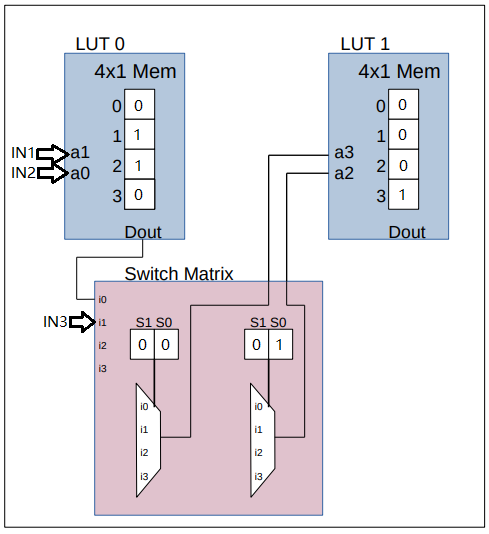
\includegraphics[width=0.5\textwidth]{Q1a.PNG}
            \caption{Q1)a}
        \end{figure}
        
        \newpage
        
        \item %b
        
        Bitstream will be 011000010001. Using the programming chain in Figure 2. The programming chain starts from the top left.
        
        \begin{figure}[ht]
            \centering
            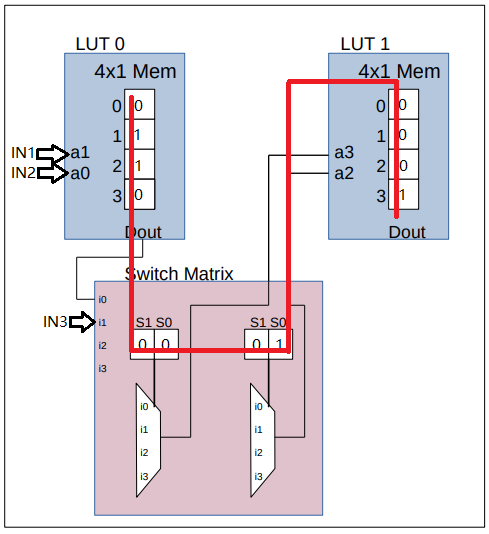
\includegraphics[width=0.5\textwidth]{Q1b.PNG}
            \caption{Q1)a}
        \end{figure}
        
    \end{enumerate}
    
    \item %Q2
    
    \begin{enumerate}
        
        \item %a
        
        \item %b
        
    \end{enumerate}
    
    \item %Q3
    
\end{enumerate}

\end{document}
